% TEMPLATE for Usenix papers, specifically to meet requirements of
%  USENIX '05
% originally a template for producing IEEE-format articles using LaTeX.
%   written by Matthew Ward, CS Department, Worcester Polytechnic Institute.
% adapted by David Beazley for his excellent SWIG paper in Proceedings,
%   Tcl 96
% turned into a smartass generic template by De Clarke, with thanks to
%   both the above pioneers
% use at your own risk.  Complaints to /dev/null.
% make it two column with no page numbering, default is 10 point

% Munged by Fred Douglis <douglis@research.att.com> 10/97 to separate
% the .sty file from the LaTeX source template, so that people can
% more easily include the .sty file into an existing document.  Also
% changed to more closely follow the style guidelines as represented
% by the Word sample file. 

% Note that since 2010, USENIX does not require endnotes. If you want
% foot of page notes, don't include the endnotes package in the 
% usepackage command, below.

% This version uses the latex2e styles, not the very ancient 2.09 stuff.
\documentclass[letterpaper,twocolumn,10pt]{article}
\usepackage{usenix,epsfig,endnotes}
\usepackage{amsmath}
\usepackage{comment}
\usepackage{url}
\usepackage{soul}
\begin{document}

\renewcommand{\ttdefault}{cmtt}

%don't want date printed
\date{}

%make title bold and 14 pt font (Latex default is non-bold, 16 pt)
\title{\Large \bf
Gdev: First-Class GPU Resource Management in the Operating System
}

%for single author (just remove % characters)
\author{
{\rm Shinpei Kato,
Michael McThrow,
Carlos Maltzahn,
and Scott Brandt
}\\
Department of Computer Science, UC Santa Cruz
%\and
%{\rm Second Name}\\
%Second Institution
% copy the following lines to add more authors
% \and
% {\rm Name}\\
%Name Institution
} % end author

\maketitle

% Use the following at camera-ready time to suppress page numbers.
% Comment it out when you first submit the paper for review.
\thispagestyle{empty}
\pagestyle{empty}

\begin{abstract}
 The graphics processing unit (GPU) has become a very powerful platform
 embracing a concept of heterogeneous many-core computing.
 Despite its significant benefits in performance, however, the
 application domains of GPUs are currently limited, largely due to
 a lack of resource management primitives to support the GPU in
 general-purpose time-sharing systems.

 In this paper, we present Gdev, a new approach to GPU resource
 management in the operating system (OS), which allows user-space
 applications and the OS itself to use the GPU as first-class computing
 resources.
 Gdev integrates runtime support into the OS, coordinated
 with the device driver to extend a class of applications that
 can benefit from the GPU.
 This runtime-unified approach also enhances the
 memory management and scheduling of GPU applications.
 Specifically, Gdev supports shared memory for inter-process
 communication among GPU contexts and data allocation beyond the
 physical device memory space.
 Scheduling is also provided to control GPU resource usage with regards
 to computations and data transmissions.
 Gdev further enables the GPU to be virtualized into logical GPUs,
 isolating a certain potion of GPU resources from other time-sharing
 users.

 We implement an open-source prototype of Gdev for Linux on NVIDIA
 GPUs, and identify the advantage and disadvantage of using Gdev,
 compared to proprietary software and previous work.
 Our detailed experiments show that Gdev can, for instance, gain about
 2x speedups for OS filesystem encryption by using the GPU, improve the
 makespans of data-flow programs by up to 50\%, and maintain virtual
 GPUs utilization within an error of 10\%.
 %While some performance loss is observed in running a standalone
 %user-space program, 

 
\end{abstract}
\section{Introduction}
\label{sec:introduction}

Even with GPU programming support in the current state of the arts, 

Existing OS-level solutions still rely on user-space runtime
engines, which provide application programming interfaces (APIs), to
generate GPU commands, and hence they never allow OSes directly to use
GPUs as first-class compute resources.
Those existing solutions also lack support for virtual memory
management, inter-process communication, and resource partitioning in
multi-tasking environments.

\cite{Kato_RTSS11}.
\section{System Model}
\label{sec:model}

This paper focuses on a system composed of a GPU and a multi-core CPU.
GPU applications use a set of the API supported by the system, and
typically take the following steps:
(i) allocate space to the device memory, 
(ii) move data to the allocated space on the device memory, 
(iii) launch computation on the GPU, 
(iv) move resultant data back to the host memory, and 
(v) free the allocated space from the device memory.
%This is the most well-known GPU programming model.
We also assume that the GPU is based on NVIDIA's \textit{Fermi}
architecture~\cite{Fermi}.
The concept of Gdev, however, is not limited to Fermi, but is also
applicable to others if the following model is applicable.

\textbf{Command:}
The GPU is operated by commands.
The commands are architecture-specific.
Each GPU context is assigned a FIFO queue, where CPU host programs push
GPU commands.
When the GPU dispatches these commands, the corresponding context can
execute. 

\textbf{Channel:}
Each GPU context is assigned a hardware channel.
Command dispatching and context execution are managed per channel.
In Fermi architecture, multiple channels cannot run simultaneously when
using the same GPU funtional unit, while they can when using different
units.
However, they are allowed to coexist, and the GPU switches the channels
automatically in hardware.

\textbf{Address Space:}
Each GPU context runs in separate virtual address space, which is also
associated with the channel.
The device driver is in charge of setting page tables for the memory
management unit on the GPU.

\begin{comment}
\textbf{I/O Register:}
The GPU provides a bunch of memory-mapped I/O registers per context
visible to the device driver through the (PCI) I/O bus.
The device driver needs to manage these registers to send commands and
set up channels and address space.
\end{comment}

\textbf{Compute Unit:}
The GPU maps the threads assined by programmers onto the compute cores.
This thread assignment, however, is not visible to the CPU.
Hence, GPU resource management by the system should be
context-based. 
Multiple contexts cannot run on the same compute unit at once, since
multiple channels cannot access the same functional unit simultaneously,
though multiple instances spawned from the same context can run.
GPU computation is also non-preemptive.

\textbf{DMA Unit:}
There are two types of DMA units for data transmission: (i) synchronous
with compute units and (ii) asynchronous.
Only the latter type of DMA units can overlap their operations with the
compute unit.
%For some reason, however, synchronous DMA is faster than asynchronous one.
DMA data transmission is also non-preemptive.

\vspace{-0.25em}
\section{Gdev Ecosystem}
\label{sec:ecosystem}
\vspace{-0.25em}

\begin{figure}[t]
 \begin{center}
  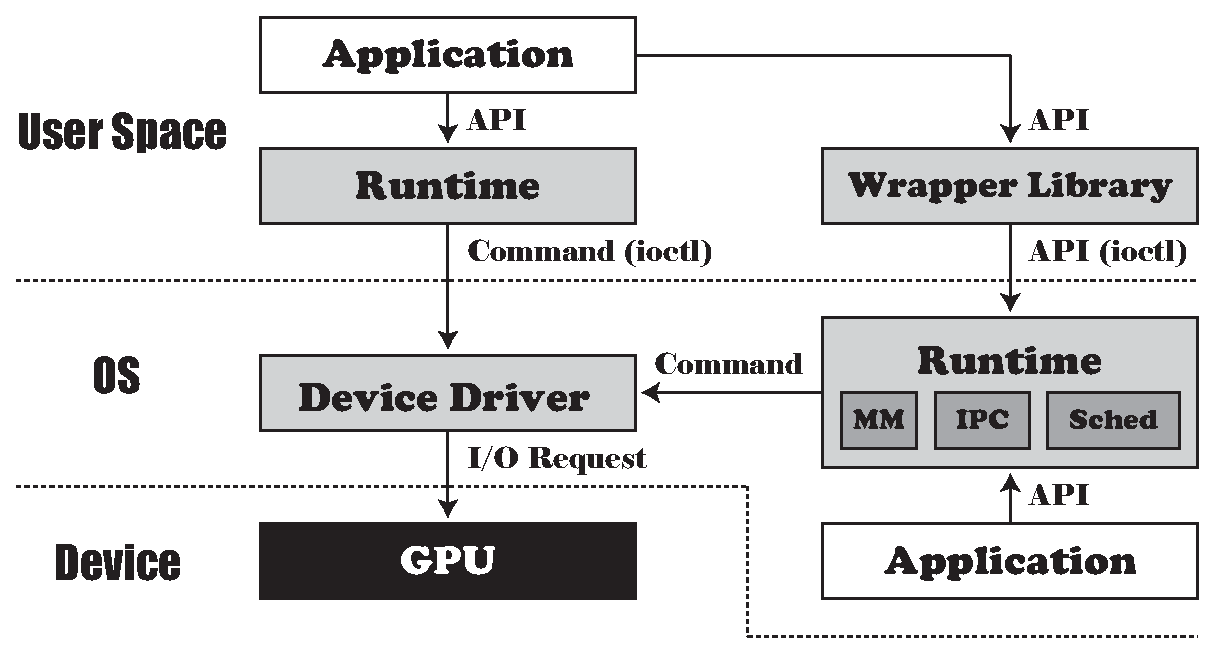
\includegraphics[width=\hsize]{eps/gdev.eps}\\
  \vspace{-0.5em}
  \caption{Logical view of Gdev's ecosystem.}
  \label{fig:gdev}
 \end{center}
 \vspace{-1.5em}
\end{figure}

Gdev aims to enhance GPU resource management, and extend a class
of applications that can use GPUs.
To this end, it integrates the major part of runtime support into the OS.
Figure~\ref{fig:gdev} illustrates the logical view of Gdev's ecosystem.
We still support a traditional execution model where applications make
API calls to the complete user-space runtime library, but this is an
optional path left for compatibility, and the system designer may
disable it to remove the reliability concern discussed in
Section~\ref{sec:introduction}.
In contrast, Gdev's runtime system resides in the OS, which enables both
user-space and OS-space applications to use the same runtime API set
protected by the OS.
Therefore, non-privileged user-space programs can never bypass the
runtime system with GPU resource management.
There is a wrapper library required for user-space applications, but this is a
tiny piece of software that simply relays API calls to the runtime
system in the OS.

Leveraging this ecosystem, we design an API-driven GPU resource
management scheme.
Figure~\ref{fig:gdev} shows that Gdev allows the OS to manage
API calls, whereas the traditional model translates API calls to GPU
commands before the OS receives them.
As discussed in previous work~\cite{Kato_ATC11}, it is very hard to
analyze GPU commands and recognize the corresponding API calls in the
OS.
Hence, the existing GPU resource management schemes in the
OS~\cite{Bautin_MCNC08, Kato_ATC11} compromise overhead to invoke the
scheduler at every GPU command submission, unless an additional
programming abstraction is provided~\cite{Rossbach_SOSP11}.
On the other hand, Gdev can manage GPU resources along with API calls,
without any additional programming abstractions.

\textbf{Programming Model:}
We provide a set of low-level functions called Gdev API for GPU
programming.
Gdev API can be a useful backend for high-level APIs, such as CUDA,
OpenCL, and HMPP.
The detail of Gdev API can be found at our website~\cite{Gdev}.
Programmers may use either Gdev API directly or a high-level API built
on top of Gdev API.
In this paper, we particularly assume that programmers use ``CUDA Driver
API 4.0''~\cite{CUDA40}.

Gdev uses an existing programming framework and commodity compiler, such
as NVIDIA CUDA Compiler (NVCC)~\cite{CUDA40}.
When a program is compiled, two pieces of binary are generated.
One executes on the CPU, and loads the other binary onto the GPU.
The CPU binary is provided as an executable file or loadable module,
while the GPU binary is an object file.
Hence, both user-space and OS-space applications can use the same
framework: (i) read the GPU binary file and (ii) load it onto the GPU.
The detailed information embedded in the object file, such as code,
static data, stack size, local memory size, and parameter format, may
depend on the programming language, but the framework does not depend on
it once the object file is parsed.

\textbf{Resource Management:}
We provide device memory management and GPU scheduling schemes to manage
GPUs as first-class computing resources.
Specifically, we provide shared device memory for IPC, data swap for
large memory demands, resource-based queuing for throughput, and
bandwidth-aware resource partitioning for virtual GPU isolation.
Since some of these features require access to low-level system
information, such as I/O regions, DMA pages, and task control blocks, it
is not straightforward for the traditional user-space runtime system to
manage these pieces of information.
Hence, we claim that Gdev is a suitable approach to first-class GPU
resource management.
The concept of Gdev is also not limited to GPUs, but can be
generalized for a broad class of heterogeneous compute devices.


\section{Device Memory Management}
\label{sec:memory_management}

Gdev manages the device memory using the virtual memory management unit
of the GPU.
%We store a page table for each GPU context in the device memory but not
%in the host memory to reduce paging latency. 
%For every memory copy operation, Gdev configures DMA engines to write a
%sequential value to the specified memory area so that it can poll the
%value to wait for the operations to be completed.
In addition to generic pieces of memory management, Gdev
identifies how to increase memory-copy throughput and support shared
memory and memory swapping for the GPU.

\subsection{Memory-Copy Optimization}
\label{sec:memory_copy}

Given that GPU applications copy data back and forth between the device
and host memory, the memory-copy throughput govern application
performance.
Though our goal is to enhance GPU resource management in time-sharing
systems, the standalone application performance is still an 
important factor to sell the practicality of our solution in the
real world.
We therefore identify how to optimize memory-copy throught for GPU
applications.
\begin{comment}
It should be noted that our problem is different from those considered
in previous work~\cite{Jablin_PLDI11, Rossbach_SOSP11} in that we are
looking into a basic single instance of memory-copy transaction, while
the previous work addressed more applied situations where multiple
contexts compete for memory-copy transaction.

First of all, we have found that the memory-copy API functions provided
by proprietary software~\cite{CUDA40} are well-optimized for standalone
operations.
In the following, hence, we disclose how to realize this optimization.
\end{comment}

\textbf{Split Transaction:}
In order to copy data between the device and host memory, the data
typically need to be copied twice, unless users directly allocate
buffers to the host I/O memory. 
For example, when uploading user buffers from the host to the device
memory, the data are first copied from the main memory to intermediate
\textit{bounce} buffers in the I/O memory accessible to the GPU, and
then copied to the device memory.
To optimize this two-step memor-copy operation, we split each operation
by a fixed size of chunks, which play a role of ping-pong buffers.
While some chunk is copied between the main and I/O memory, the prior
chunk can be copied between the I/O and device memory.
In this way, only the first and last chunks are copied alone, while
others are overlapped with neighbors, reducing the makespan almost half.
This split transaction also needs only a small size of bounce buffers
equal to the chunk size, reducing the usage of the host I/O memory
significantly.
%In Gdev, the chunk size is configurable.
%The same idea can also be applied to all types of DMA engines desribed in
%Section~\ref{sec:model}.

\textbf{Direct I/O Access:}
The split transaction is effective for a large size of data.
For a small size of data, however, the use of DMA engines incurs
non-trivial overhead by itself.
Hence, we also employ a method to directly map device memory space onto
host I/O memory space and read/write data sequentially rather than
configure DMA engines and send/receive data in burst mode.
We have found that such a direct I/O access method is much faster than
using DMA engines for a small size of data.
In our experiment presented in Section~\ref{sec:evaluation}, we will
show a boundary on the data size that inverts the surperiority of I/O
access and DMA, together with the best chunk size, to achieve
memory-copy optimization.

\subsection{Shared Memory Support}
\label{sec:shared_memory}

The current GPU programming model does not support IPC.
For example, data communication among contexts incurs significant
overhead by copying data back and forth between host-memory and
device-memory buffers.
Currently, an OS dataflow abstraction~\cite{Rossbach_SOSP11} is a useful
tool to minimize such data movement costs; however users are required to
use a dataflow programming model and understand that optimization is
applied implicitly by the OS at runtime.
It would be nice if users could manage data communiation among contexts
easily using a familiar method, such as a POSIX IPC mechanism.

Gdev supports shared memory for the GPU, providing a set of API
functions, as listed in Table~\ref{tab:gdev_api}, based on the POSIX IPC
standard, \textit{i.e.}, \texttt{gshmget}, \texttt{gshmat},
\texttt{gshmdt}, and \texttt{gshmctl} correspond to \texttt{shmget},
\texttt{shmat}, \texttt{shmdt}, and \texttt{shmctl} respectively.
We have also added \texttt{cuShmGet}, \texttt{cuShmAt},
\texttt{cuShmDt}, and \texttt{cuShmCtl} to our CUDA API 
implementation, which correspondingly call the Gdev shared memory
functions, so that CUDA applications can easily leverage Gdev's shared
memory support.

Our shared memory design is straightforward, though its implementation
is challenging.
Upon the first call to \texttt{gshmget}, new space is allocated to the
device memory, similar to \texttt{gmalloc}, and it holds an identifier
to this memory object. 
After the first call, however, Gdev only returns this identifier to the
caller.
The allocated space is mapped onto the context virtual address space
when \texttt{gshmat} is called.
Address mapping is done by setting the page table so that the virtual
addresses point to the shared physical memory space.
The allocated space can also be unmapped by \texttt{gshmdt} and freed by
\texttt{gshmctl}. 
Gdev counts the number of users for each shared memory space,
and frees the shared memory when the nubmer of references becomes zero.
Hence the call to \texttt{gshmctl} is optional.
If the shared memory needs to be accessed exclusively, the host program
must take care of it by itself using traditional semaphore mechanisms.

We believe that our shared memory scheme can be easily integrated into
GPU programing.
For example, legacy CUDA applications can use our shared memory scheme
by replacing \texttt{cuMemAlloc} with \texttt{cuShmGet} and
\texttt{cuShmAt}, and \texttt{cuMemFree} with \texttt{cuShmDt}.

\subsection{Memory Swapping}
\label{sec:memory_swapping}

The proprietary software in Linux~\cite{CUDA40} fails to allocate
device memory, when the demand exceeds the physical space, though
that in Windows can somehow allocate memory larger than the physical
memory, according to PTask~\cite{Rossbach_SOSP11}. 
In either case, however, it is not well studied how to swap device
memory and speed up its operation.

Gdev uses shared memory to achieve device memory swapping.
When a memory allocation request fails due to a short of free memory
space, Gdev seeks memory objects whose allocated size is greater than
the requested size, and selects one owned by a low-priority context,
where ties are broken arbitrarily.
Gdev here ensures not to select a memory object from the caller context
itself.
Once a victim memory object is selected, it is shared with the caller
context, and behaves as an \textit{implicit} shared memory object.
%The allocated space is never freed until unreferenced by all associated
%contexts.
Unlike an explicit shared memory object presented in
Section~\ref{sec:shared_memory}, however, the implicit shared memory
object needs to evict data when other contexts are accessing it and
retrieve the evicted data later when the corresponding context is
resumed.
Thanks to the Gdev API design, we know exactly when contexts could
access the shared memory: it could be accessed when either a familiy of
\texttt{gmemcpy*} or \texttt{glaunch} is called.
They however need to be handled in a different manner:
\begin{itemize}
 \vspace{-0.25em}
 \item \texttt{gmemcpy*} accesses a specific range of address space
       given by the function arguments.
       Hence, we need to evict and retrieve data related to this range.
 \vspace{-0.5em}
 \item \texttt{glaunch}, on the other hand, does not tell which address
       range could be accessed when it is called, especially due to
       dynamically allocated memory space.
       Hence, we need to evict and retrieve data associated with all
       memory objects owned by the corresponding context.
 \vspace{-0.25em}
\end{itemize}

We allocate swap buffers to the host main memory to save the evicted
data.
It uses \texttt{gmemcpy\_from\_device} and \texttt{gmemcpy\_to\_device}
to evict and retrieve data.
These memory swapping procedures are not visible to application programs.
It should be noted that swapping does not occur when downloading data
from the device memory.
Even if the data are evicted, we can copy the data from the host swap
buffer directly.

\textbf{Reducing Latency:}
The swapping latency could be non-trivial depending on the data size.
Given memory copy operations within the device memory faster than
those between the device and host memory by an order of ten, Gdev
reserves a certain amount of device memory space to use as temporal swap
space.
Data can be evicted to this device swap space temporarily, if the data
fit the space, to reduce the swapping latency.
The temporarily-evicted data are eventually evicted to the host memory
after a while to free the swap space for other contexts.
Gdev tries to hide the latency of this second data eviction by
overlapping it with the computation launched by the context itself.
To do so, it creates a special GPU context that copies data to the host
memory, as the compute and DMA units can be used only by different
CPU contexts simultaneously, as explained in Section~\ref{sec:model}.
This approach is reasonable, since some computation is likely following
the data eviction.
For example, \texttt{glaunch} will apparently launch some computation, and
\texttt{gmemcpy\_to\_device} is also often called prior to \texttt{glaunch}.


The evicted data, if exist, need to be retrieved when \texttt{glaunch}
is called for the associated GPU context after evicting the current data
of some other context sharing the memory space.
If the evicted data still exist in the device swap space, they can be
retrieved quickly.
Else, Gdev retrieves them from the host main memory.

\section{GPU Scheduling}
\label{sec:scheduling}

The goal of the Gdev scheduler is to assign computation and data
transmission times for GPU contexts correctly based on the given
scheduling policy.
Although we make use of some previous
techniques~\cite{Kato_RTSS11,Kato_ATC11}, Gdev provides a new context
queuing scheme and virtual GPU support for general-purpose time-sharing
systems.

\subsection{Scheduling and Queuing}
\label{sec:scheduling_queueing}

Gdev uses a simiar scheme to TimeGraph~\cite{Kato_ATC11} for GPU
scheduling.
Specifically, it allows GPU contexts to use GPU resources only if no
other contexts are using the corresponding resources.
The pending GPU contexts are queued by the scheduler while waiting for
the current context holding the resources.
To notify the completion of the current context execution, Gdev
uses additional GPU commands to generate an interrupt from the GPU.
The highest-priority context is chosen from the queue upon every
interrupt, and dispatched to the GPU.
The computation and data transmission times are separately measured and
accumulated for resource accounting.
For compute requests, we also allow the same context to launch compute
instances simultaneously, and the total makespan from the first to the last
instance is deemed as the computation time.
PTask~\cite{Rossbach_SOSP11} and RGEM~\cite{Kato_RTSS11} also use
similar mechanisms, but do not use interrupts, and thereby resource
accounting is managed by the user space via the API.

The difference between Gdev and TimeGraph is that Gdev is API-driven,
invoking a scheduler only when \texttt{gmemcpy*} or \texttt{glaunch} is
called, while TimeGraph is command-driven, invoking a scheduler whenever
GPU commands are flushed.
In this regard, Gdev is similar to PTask~\cite{Rossbach_SOSP11} and
RGEM~\cite{Kato_RTSS11}.
However, Gdev differs even from these prior work in that it supports
separate queues for resource accounting of compute and memory-copy
operations, which we call \textit{Multiple Resource Queues} (MRQ), while
we call \textit{Single Device Queue} (SDQ) for the previous approach
where the scheduler supports only a single queue per device for resource
accounting.

The MRQ scheme is apparently more efficient than the SDQ scheme, when
different compute and memory-copy operations can be overlapped.
Suppose that there are two contexts both requesting 50\% of compute
and 50\% of memory-copy demands.
The SDQ scheme considers that the demand of each context is 100\% by
adding compute and memory-copy demands, and the total demand of the
two context is 200\%.
This workload thereby looks overloaded under the SDQ scheme.
The MRQ scheme, on the other hand, does not consider the total workload
to be overloaded while each resource to be fully utilized.

Gdev creates different scheduler threads for compute and memory-copy
operations. 
The compute scheduler thread is invoked upon the associated interrupt
generated by the GPU, while the memory-copy scheduler thread is awakened
by the Gdev runtime when the memory-copy operation is done, since we do
not use interrupts for memory-copy operations.

Priority assignments are focused on in this paper.
Gdev simply propagates the task priority, assigned by the OS, to the
corresponding GPU context. 

\subsection{Virtual GPU Support}
\label{sec:virtual_gpu}

Gdev is capable of partitining the time and space of the GPU to
virtualize a physical GPU to logical GPUs.
Users accessing different virtual GPUs are not interfered with each
other.
Virtual GPUs are activated by specifying the weights of GPU resources
assigned to each of them.
We classify GPU resources into the \textit{memory share}, \textit{memory
bandwidth}, and \textit{compute bandwidth}.
The memory share is the weight of the physical memory space available
for the virtual GPU, and Gdev simply reserves the physical memory space
in accordance with the specified memory share.
The memory bandwidth is the amount of time per some period given for
memory-copy operations related to the GPU, and the compute bandwidth is
that for GPU compute operations.
Gdev creates compute and memory-copy scheduler threads for each virtual
GPU.
The system comprising 4 virtual GPUs, for example, would contain 8
instances of the Gdev scheduler in total.
We however apply the same scheduling policy to the compute and
memory-copy schedulers.

The challenge for virtual GPU scheduling is raised by the non-preemptive
and burst nature of GPU workloads.
We have implemented the Credit scheduling algorithm supported by Xen
hypervisor~\cite{Barham_SOSP03} to verify if an existing virtual CPU
scheduling policy can be applied for a virtual GPU scheduler.
However, we have found that the Credit scheduler fails to maintain the
desired bandwidth for the virtual GPU, largely attributed to the fact
that it presumes preemptive constantly-working CPU workloads, while GPU
workloads are non-preemptive and bursting.

\begin{figure}[t]
 \begin{center}
  \begin{tabular}{l}
   \hline
   \hline
   {\small \verb|vgpu->bgt|: budget of the virtual GPU.}\\
   {\small \verb|vgpu->utl|: actual GPU utilization of the virtual GPU.}\\
   {\small \verb|vgpu->bw|: bandwidth assigned to the virtual
   GPU.}\\
   {\small \verb|current/next|: current/next virtual GPU selected for run.}\\
   \hline
   {\small \verb|void on_arrival(vgpu, ctx) {|}\\
   {\small \verb|  if (current && current != vgpu)|}\\
   {\small \verb|    suspend(ctx);|}\\
   {\small \verb|  dispatch(ctx);|}\\
   {\small \verb|}|}\\
   {\small \verb|vgpu_instace* on_completion(vgpu, ctx) {|}\\
   {\small \verb|  if (vgpu->bgt < 0 && vgpu->utl > vgpu->bw)|}\\
   {\small \verb|    move_to_queue_tail(vgpu);|}\\
   {\small \verb|  next = get_queue_head();|}\\
   {\small \verb|  if (!next) return null;|}\\
   {\small \verb|  if (next != vgpu && next->utl > next->bw) {|}\\
   {\small \verb|    wait_for_short();|}\\
   {\small \verb|    if (!current) return next;|}\\
   {\small \verb|    else return null;|}\\
   {\small \verb|  }|}\\
   {\small \verb|}|}\\
   \hline
  \end{tabular}
  \caption{Pseudo-code of the Band scheduler.}
  \label{fig:band}
 \end{center}
 \vspace{-1.5em}
\end{figure}

To overcome the virtual GPU scheduling problem, we propose a
\textit{bandwidth-aware non-preemptive device} (Band) scheduling
algorithm.
The pseudo-code of the Band scheduler is shown in
Figure~\ref{fig:band}.
The \texttt{on\_arrival} function is invoked by the task associated with
a context \texttt{ctx} assigned to a virtual GPU \texttt{vgpu} when
it is about to use GPU resources.
The context can be dispatched to the GPU only if no other virtual GPUs
are holding the GPU.
Otherwise, the corresponding task is suspended.
On the other hand, the \texttt{on\_completion} functions is called by
the corresponding scheduler thread upon the completion of a context
\texttt{ctx} assined to a virtual GPU \texttt{vgpu}, to select the next
virtual GPU to execute. 
Our scheduling policy is based on the Credit scheduler but differs in
the following two points.
First, the Band scheduler lowers the priority of the virtual GPU when
its budget (credit) is exhausted and its utilization of the GPU is
exceeding the assigned bandwidth, while the Credit scheduler always
lowers the priority when the budget is exhausted.

The second modification to the Credit scheduler is that the Band
scheduler waits for a certain amount of time specified by the system
designer, if the GPU utilization of the virtual GPU selected
by the scheduler is exceeding its assigned bandwidth.
This particularly works for non-preemptive burst workloads.
Suppose that the system has two virtual GPUs, both of which execute
burst workloads with some contexts, but each non-preemptive execution
has a different length.
If their contexts arrive in turn, they are also dispatched to the GPU in
turn, but the GPU utilization could not be fair due to different lengths
of non-preemptive executions.
If the scheduler waits for a short interval, however, the context with a
short length of non-preemptive execution could arrive with the next
request, and the \texttt{on\_arrival} function can dispatch it to the
GPU while the scheduler is waiting.
In such a case, the scheduler needs not to select the next virtual
GPU, as the \texttt{on\_arrival} function has already dispatched the
context.
Otherwise, it returns the selected virtual GPU.
If the context does not arrive while the scheduler is waiting, it
implies that this is not a burst workload, and hence is not emergent to
meet the bandwidth.

\section{System Implementation}
\label{sec:implementation}

Our prototype implementation is fully open-source and available for the
Linux kernel 2.6.32 or later, without any modifications to the
underlying kernel, on NVIDIA Fermi GPUs.
It does not depend on proprietary software except for compilers.
%Our device driver implementation is particularly based on what we have
%been developing in collaboration with PathScale
%Corporation~\cite{ENZO}.
%The OS runtime and the CUDA Driver API library, on the other hand, are
%newly implemented.
Our prototype implementation is still partly experimental, but it could
contribute to future research on GPU resource management, given that
open-source drivers/runtimes for GPUs has not appeared yet.

\textbf{Interface:}
Gdev is a Linux kernel module (a character device driver) composing the
device driver and runtime library.
The device driver manages low-level hardware resources, such as channels
and page tables, to operate the GPU.
The runtime library manages GPU commands and API calls.
It directly uses the device-driver functions to control hardware
resource usage for first-class GPU resource management.
The Gdev API is implemented in this runtime library.
The kernel sympols of the API functions are exported so that other OS
modules can call them.
These API functions are also one-to-one mapped to the \texttt{ioctl}
commands defined by Gdev so that user-space programs can also be managed
by Gdev.

Simiar to Gdev API, we provide two versions of CUDA Driver API: one for
the user space and the other for the OS.
The former is provided as a typeical user-space library, while the
latter is provided as a kernel module, called \textit{kcuda},
which implements and exports the CUDA API functions.
They however internally use Gdev API to access the GPU.

We use \texttt{/proc} filesystem in Linux to configure Gdev.
For example, the number of virtual GPUs and their maps to physical GPUs
are visible to users through \texttt{/proc}.
The compute and memory bandwidth and memory share for each virtual GPU
are also configurable at runtime through \texttt{/proc}.
We further plan to integrate the configuration of priority and
reserve for each single task into \texttt{/proc}, using the TimeGraph
approach~\cite{Kato_ATC11}.

Gdev creates the same number of character device files as virtual GPUs,
\textit{i.e.}, /dev/\{gdev0,gdev1,...\}.
When users open one of these device files using Gdev API or CUDA API,
it behaves as if it were one for the physical GPU.

\textbf{Resource Parameters:}
The performance of Gdev is governed by resource parameters, such as the
page size for virtual memory, temporal swap size, waiting time for the
Band scheduler, period for virtual GPU budgets, chunk size
for memory-copy, and boundary between I/O access and DMA.
We use a page size of 4KB, as the Linux kernel uses the same page size
for host virtual memory by default.
The swap size is statically set 10\% of the physical device memory.
The waiting time for the Band scheduler is also statically set 500
microseconds.
For the period of virtual GPU budgets, we respect Xen's default setup,
\textit{i.e.}, we set it 30ms.
The rest of resource parameters will be determined through the experiments as
demonstrated in Section~\ref{sec:evaluation}.

\textbf{Portability:}
We use Direct Rendering Infrastracture (DRI)~\cite{DRI} -- a Linux
framework for graphics rendering with the GPU -- to communiate with the
Linux kernel.
Hence, some Gdev functionality may be used to manage not only compute
but also 3-D graphics applications.
Our implementation approach also abstracts GPU resources by device,
address space, context, and memory objects, which allows other device
drivers and GPU architectures to be easily ported.
We believe that this portability would help to generalize the concept of
Gdev. 


\vspace{-0.25em}
\section{Experimental Evaluation}
\label{sec:evaluation}
\vspace{-0.25em}

We evaluate our Gdev prototype, using the Rodinia
benchmarks~\cite{Che_IISWC09}, GPU-accelerated eCryptfs encrypted
file system from KGPU~\cite{Sun_SYSTOR12}, FAST database
search~\cite{Kim_SIGMOD10}, and some dataflow
microbenchmarks from PTask~\cite{Rossbach_SOSP11}.
We disclose that the basic performance of our prototype is practical
even compared to proprietary software, and also demonstrate that Gdev
provides significant benefits for GPU applications in time-sharing
systems.

Our experiments are conducted with the Linux kernel 2.6.39 on NVIDIA
GeForce~GTX~480 graphics card and Intel Core~2~Extreme QX9650 processor.
GPU programs are written in CUDA and compiled by NVCC~\cite{CUDA40},
while CPU programs are compiled by gcc 4.4.6.

\vspace{-0.25em}
\subsection{Basic Performance}
\vspace{-0.25em}

\begin{figure}[t]
 \begin{center}
  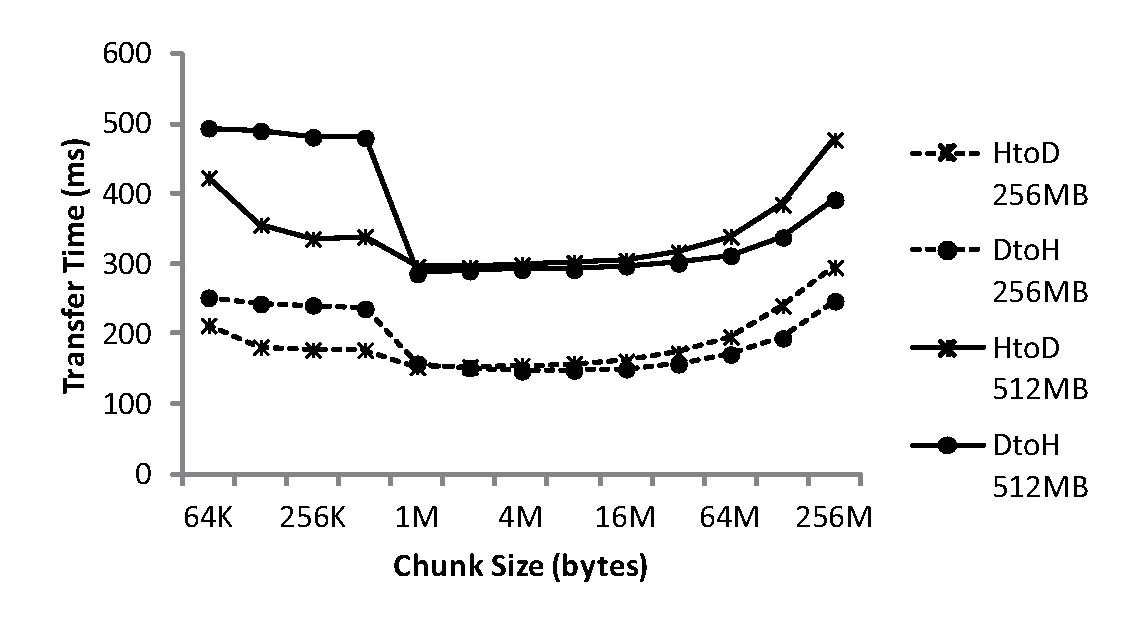
\includegraphics[width=0.8\hsize]{eps/chunk.eps}\\
  \vspace{-1.5em}
  \caption{Impact of the chunk size on DMA speeds.}
  \label{fig:chunk}
 \end{center}
 \vspace{-1.5em}
 \begin{center}
  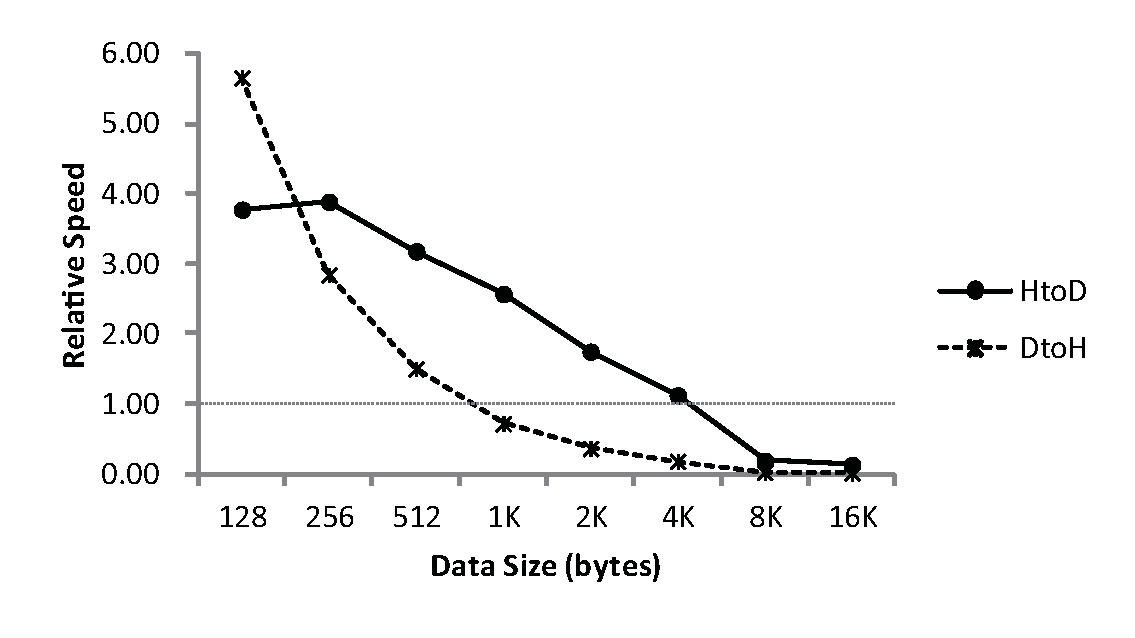
\includegraphics[width=0.8\hsize]{eps/dma.eps}\\
  \vspace{-1.5em}
  \caption{Relative speed of I/O access to DMA.}
  \label{fig:io_access}
 \end{center}
 \vspace{-1.5em}
 \begin{center}
  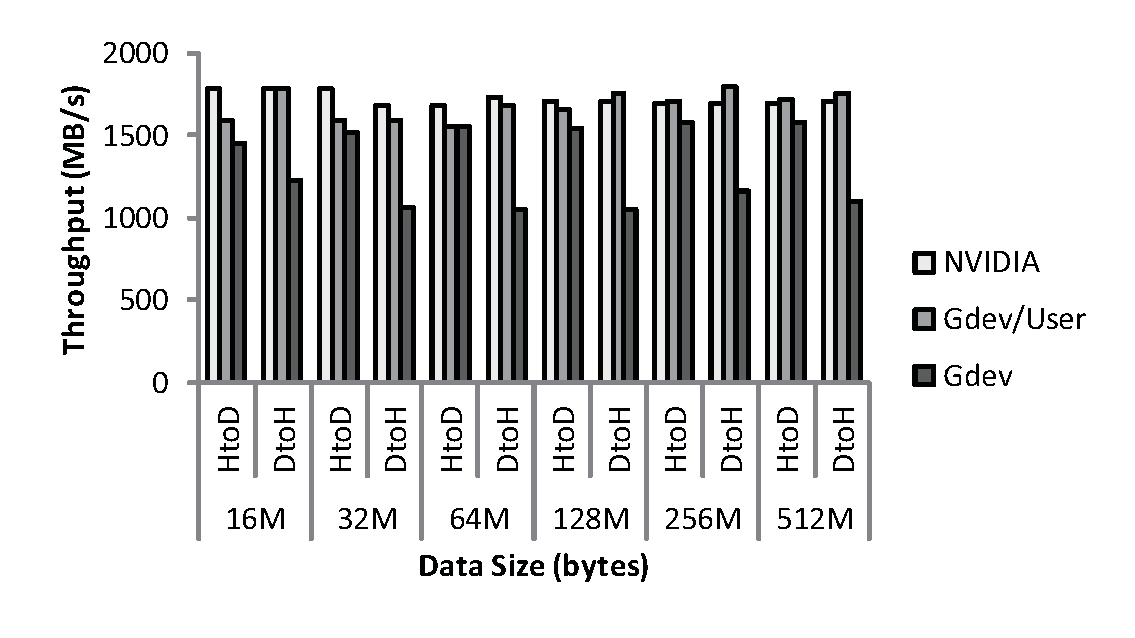
\includegraphics[width=0.9\hsize]{eps/memcpy.eps}\\
  \vspace{-1.5em}
  \caption{Memory-copy throughput.}
  \label{fig:memcpy}
 \end{center}
 \vspace{-1.5em}
\end{figure}

We evaluate the standalone performance of applications achieved by
our Gdev prototype to argue that the rest of our evaluation is practical
in the real world.
To this end, first of all, we need to find the best parameters used for
memory-copy optimization, using simple test code that copies data
between device and host memory.

Figure~\ref{fig:chunk} shows the impact of the chunk size on data
transfer times for host-to-device (HtoD) and device-to-host (DtoH)
directions respectively, when using DMA-based memory-copy operations
with 256MB and 512MB of data.
Since each chunk incurs some overhead in DMA configuration, a
smaller chunk size producing a greater number of chunks increases a
transfer time.
On the other hand, there is a constraint that the first and last pieces
of chunks cannot be overlapped with others, as described in
Section~\ref{sec:memory_copy}.
Hence, a larger chunk size leading to a longer blocking time with these
pieces of chunks also increases a transfer time.
According to our observation, a chunk size of 4MB is the best trade-off
for both HtoD and DtoH directions.
We therefore set the chunk size to 4MB for our experiments.

Figure~\ref{fig:io_access} shows the relative speed of direct I/O
access to DMA for a small size of data. 
Due to some hardware effect, HtoD and DtoH directions show different
transfer times, but it clearly explains the advantage of direct I/O
access for small data.
According to our observation, the data transfer speed inverses around a
data size of 4KB and 1KB for HtoD and DtoH directions respectively.
We therefore set the boundary of direct I/O access and DMA to 4KB and
1KB for them respectively.

Figure~\ref{fig:memcpy} shows memory-copy throughput achieved
by our Gdev prototype compared to NVIDIA's proprietary software.
``Gdev/User'' employs a runtime library in the user-space, while
``Gdev'' integrates runtime support into the OS.
Interestingly, user-space runtime achieves higher throughput than
OS-space runtime, particularly for DtoH direction.
This difference comes from \texttt{memcpy}'s effect within host memory.
In fact, the \texttt{memcpy} implementation in the Linux kernel is slower
than that in the user-space GNU library, when copying data from host I/O
to main memory.
This could be a disadvantage of our approach.
We will investigate this effect more in depth.
Apart from the DtoH memory-copy throughput, however, our Gdev prototype
and NVIDIA's proprietary software are almost competitive.
 
\begin{table}[t]
 \caption{List of benchmarks.}
 \label{tab:benchmarks}
 \vspace{-0.5em}
 \begin{center}
  {\footnotesize
  \begin{tabular}{|l|l|}
   \hline
   \textbf{Benchmark} & \textbf{Description}\\
   \hline
   LOOP & Long-loop compute without data \\
   \hline
   MADD & 1024x1024 matrix addition\\
   \hline
   MMUL & 1024x1024 matrix multiplication\\
   \hline
   CPY & 256MB of HtoD and DtoH\\
   \hline
   PINCPY & CPY using pinned host I/O memory\\
   \hline
   BP & Back propagation (pattern recognition)\\
   \hline
   BFS & Breadth-first search (graph algorithm)\\
   \hline
   HW & Heart wall (medical imaging)\\
   \hline
   HS & Hotspot (physics simulation)\\
   \hline
   LUD & LU decomposition (linear algebra)\\
   \hline
   NN & K-nearest neighbors (data mining)\\
   \hline
   NW & Needleman-wunsch (bioinformatics)\\
   \hline
   SRAD & Speckle reducing anisotropic diffusion (imaging)\\
   \hline
   SRAD2 & SRAD with random pseudo-inputs (imaging)\\
   \hline
  \end{tabular}
  }
 \end{center}
 \vspace{-1.5em}
\end{table}

Figure~\ref{fig:basic_performance} demonstrates the standalone
performance of benchmarks achieved by our Gdev prototype compared to
NVIDIA's proprietary software.
Table~\ref{tab:benchmarks} describes the microbenchmarks and
Rodinia~\cite{Che_IISWC09} benchmarks used in this evaluation.
First of all, we have found that NVIDIA GPUs have some ``performance
mode'' to boost hardware performance that we do not use for our Gdev
prototype implementation.
As observed in the LOOP benchmark result, our Gdev prototype incurs
about 20\% of decrease in performance compared to the proprietary
software due to a lack of performance mode.
However, the impact of performance mode is workload dependent.
If workloads are very compute-intensive, such as the HW and SRAD
benchmarks, this impact appears clearly, whereas some friendly
workloads, such as the BFS and HS benchmarks, are not influenced very
much.
In either case, however, this is an implementation issue, but is
not a conceptual limitation of Gdev.
These benchmark results also imply that Gdev's runtime-unified OS
approach would not be appreciated by data-intensive workloads.
For example, the BP benchmark is associated with a very large size of data,
though its compute demand is not very high.
This type of workload would not perform well with our Gdev prototype, since
the \texttt{memcpy} function of the Linux kernel becomes a bottleneck.
On the other hand, the PINCPY benchmark does not need \texttt{memcpy}
operations.
Hence, performance does not depend on implementations.

\begin{figure}[t]
 \begin{center}
  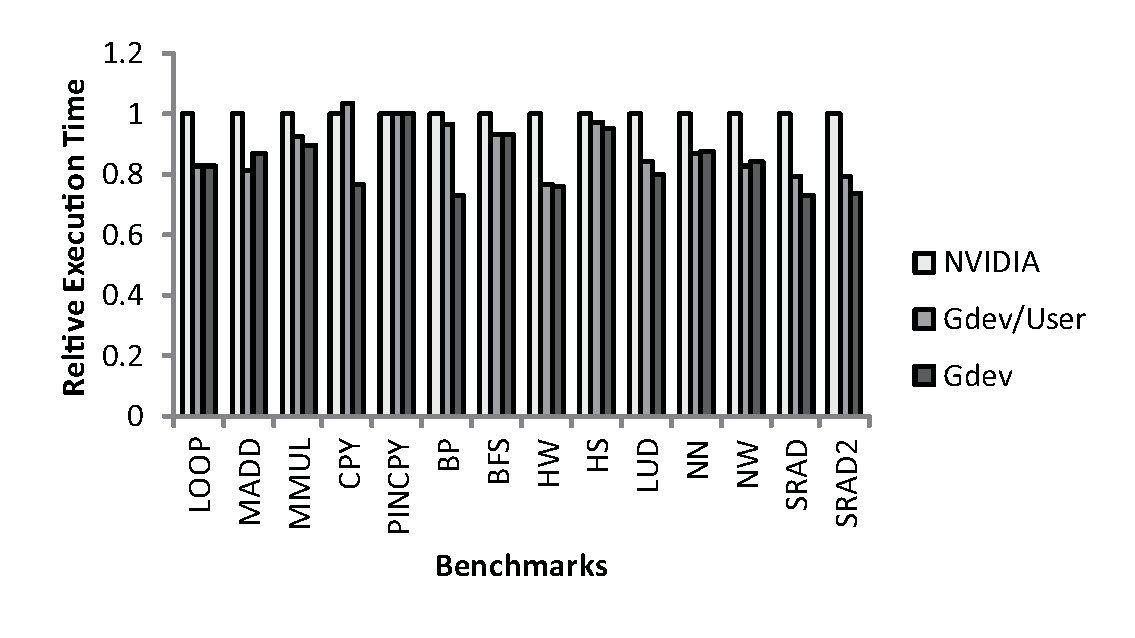
\includegraphics[width=0.9\hsize]{eps/basic_performance.eps}\\
  \vspace{-1.5em}
  \caption{Basic standalone performance.}
  \label{fig:basic_performance}
 \end{center}
 \vspace{-1.5em}
 \begin{center}
  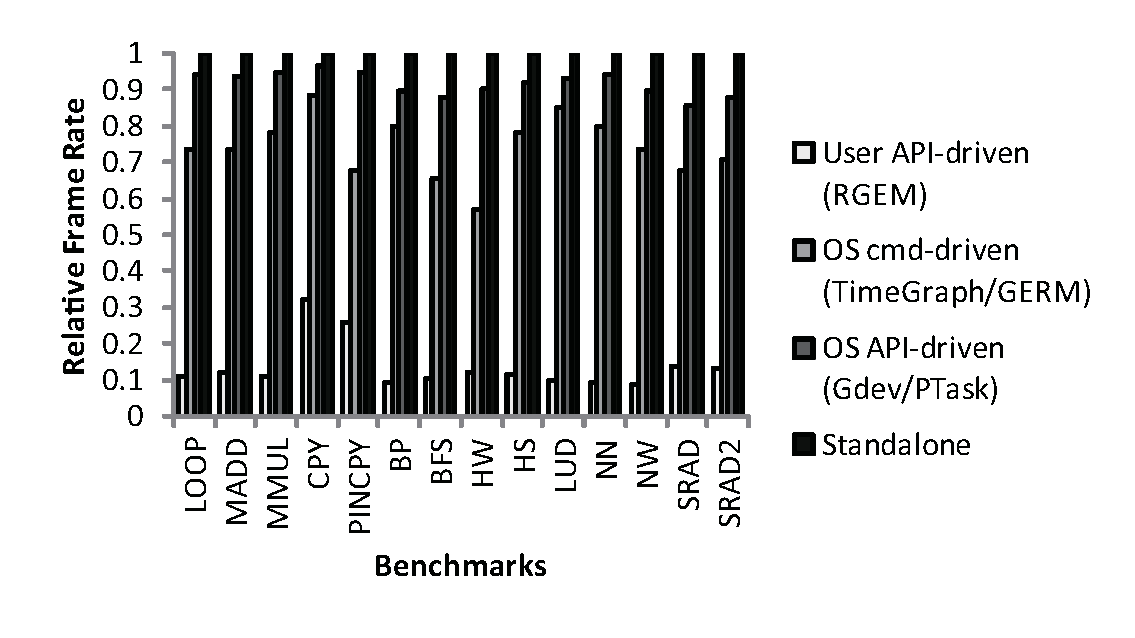
\includegraphics[width=0.9\hsize]{eps/scheduler_overhead.eps}\\
  \vspace{-1.5em}
  \caption{Unconstrained real-time performance.}
  \label{fig:scheduler_overhead}
 \end{center}
 \vspace{-1.5em}
\end{figure}

\vspace{-0.25em}
\subsection{Reliability}
\vspace{-0.25em}

We next evaluate reliability of runtime support integrated in the OS.
Figure~\ref{fig:scheduler_overhead} compares the performances of the
OS-space API-driven scheme (Gdev and PTask~\cite{Rossbach_SOSP11}),
the OS-space command-driven scheme (TimeGraph~\cite{Kato_ATC11} and
GERM~\cite{Bautin_MCNC08}), and the user-space API-driven scheme
(RGEM~\cite{Kato_RTSS11}).
We run Rodinia benchmarks recursively as fast as possible as
real-time tasks, contending with such background tasks that bypass the
user-space library and launch many meaningless GPU commands.
The user-space API-driven scheme severely suffers from this situation,
since it cannot schedule these bypassing tasks at all.
The OS-space command-driven scheme is able to sustain the interference
to some extent by using the GPU command scheduler, but the overhead is
non-trivial due to many scheduler invocations.
On the other hand, the OS-space API-driven scheme can reject such command
submission that is not submitted through the API.
Gdev and PTask are both API-driven, but PTask exposes the system call to
user-space programs, which could allow misbehaving tasks to abuse GPU
resources.
This evinces that Gdev's approach that integrates runtime support into
the OS is a more reliable solution.

\vspace{-0.25em}
\subsection{GPU Acceleration for the OS}
\vspace{-0.25em}

\begin{figure}[t]
 \begin{center}
  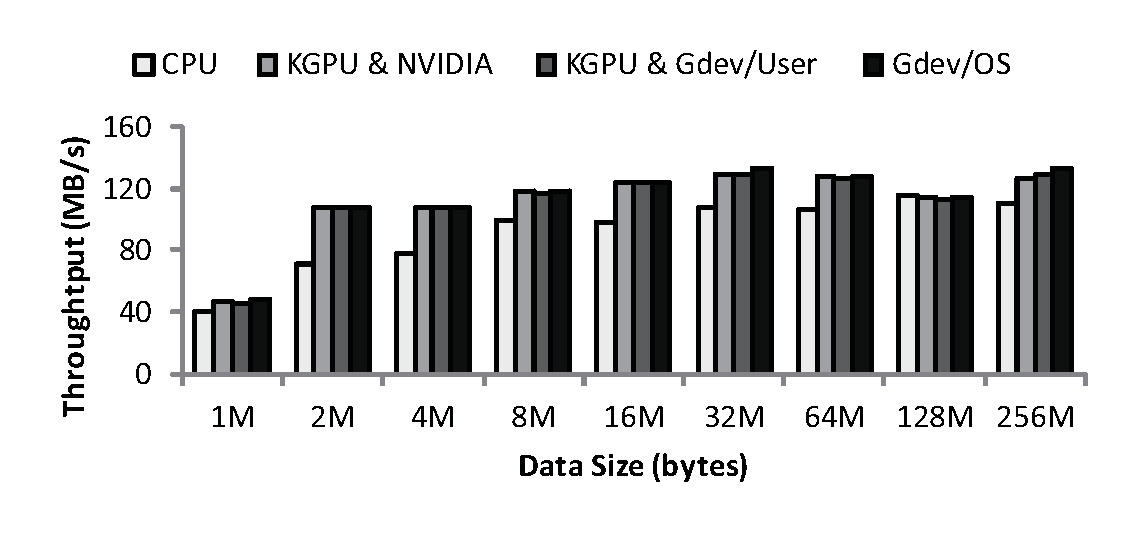
\includegraphics[width=0.9\hsize]{eps/ecryptfs_read.eps}\\
  \vspace{-1.5em}
  \caption{eCryptfs read throughput.}
  \label{fig:ecryptfs_read}
 \end{center}
 \vspace{-1.5em}
 \begin{center}
  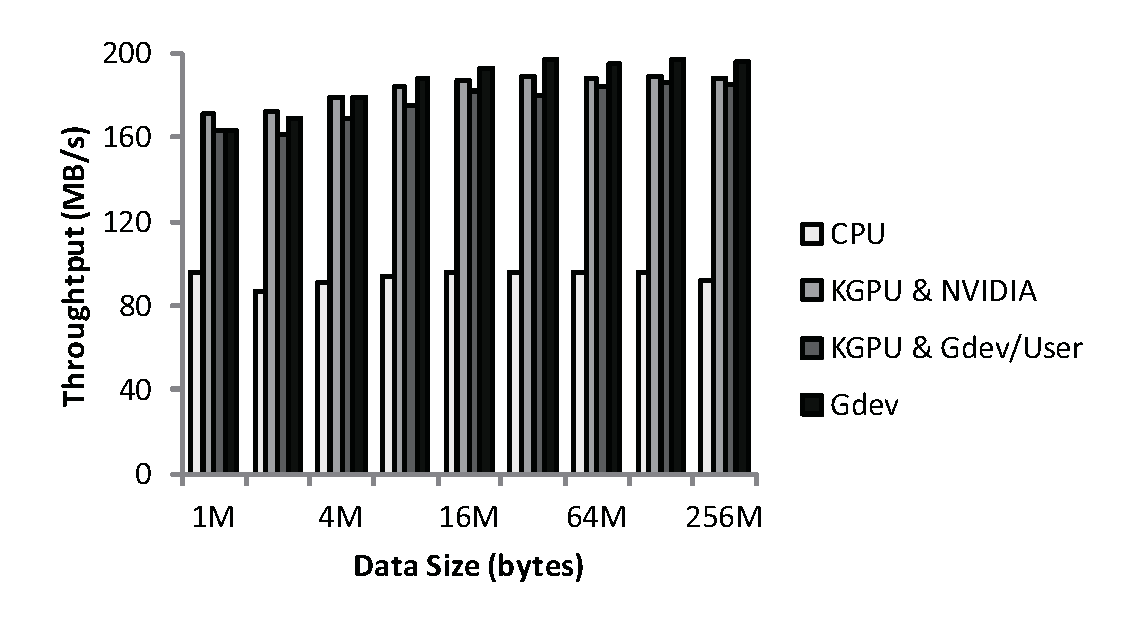
\includegraphics[width=0.9\hsize]{eps/ecryptfs_write.eps}\\
  \vspace{-1.5em}
  \caption{eCryptfs write throughput.}
  \label{fig:ecryptfs_write}
 \end{center}
 \vspace{-1.5em}
 \begin{center}
  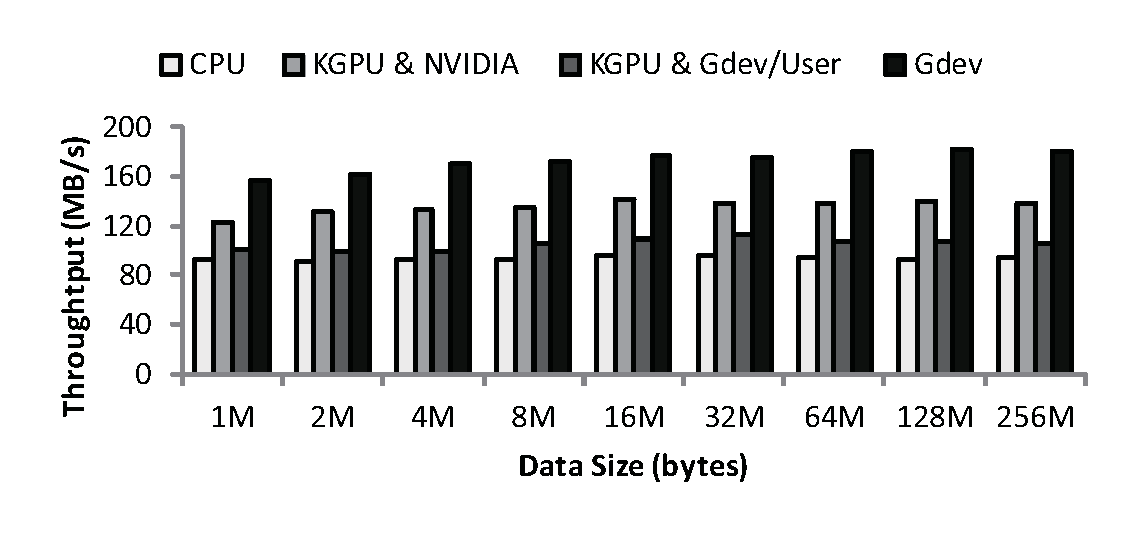
\includegraphics[width=0.9\hsize]{eps/ecryptfs_write_multitask.eps}\\
  \vspace{-1.5em}
  \caption{eCryptfs write throughput with priorities.}
  \label{fig:ecryptfs_write_multitask}
 \end{center}
 \vspace{-1.5em}
\end{figure}

We now evaluate the performance of the Linux encrypted file system
accelerated by the GPU.
In particular, we use KGPU's implementation of
eCryptfs~\cite{Sun_SYSTOR12}.
KGPU is a framework that allows the OS to access the user-space runtime
library to use GPUs for computations.
We have modified KGPU's eCryptfs implementation to call the CUDA API
functions provided by Gdev directly instead of sending requests to the
KGPU user-space daemon.

Figure~\ref{fig:ecryptfs_read} and \ref{fig:ecryptfs_write} show the
read and write throughput of several versions of eCryptfs.
``CPU'' represents the CPU implementation, while ``KGPU \& NVIDIA'' and
``KGPU \& Gdev/User'' represent those using KGPU with NVIDIA's library
and Gdev's library respectively in the user space. 
``Gdev'' is our contribution that enables the eCryptfs module to use the
GPU directly within the OS.
Due to some page cache effect, read and write are not identical in
throughput, but an advantage of using the GPU is clearly depicted.
One may observe that Gdev's runtime-unified OS approach does not really
outperform KGPU's approach.
This is not surprising at all, because a magnitude of improvements in
latency achieved by our OS approach would be at most microseconds, while
the AES/DES operations of eCryptfs performed on the GPU are
orders-of-milliseconds.
Nonetheless, Gdev provides a significant benefit that the OS is freed
from the user space, and thus is more secure.

A further advantage of using Gdev appears in a multi-tasking scenario.
Figure~\ref{fig:ecryptfs_write_multitask} shows the write throughput of
eCryptfs when the FAST search task~\cite{Kim_SIGMOD10} is competing for
the GPU.
Since Gdev supports priorities in the OS, we can assign the eCryptfs
task with the highest priority, while the search task is still assigned
a higher priority than other tasks.
Using KGPU in this scenario, however, the performance of eCryptfs is
affected by the search task due to a lack of prioritization, as observed
in ``KGPU \& NVIDIA''.
Even with priorities, KGPU could suffer from a priority inversion
problem, where the high-priority eCryptfs task is reduced to the KGPU
priority level when accessing the GPU, while the search task is
executing at the higher priority level.
We could assign a high priority to the user-space KGPU daemon to avoid
this priority inversion problem, but it affects all user-space GPU
applications performance. 
On the other hand, Gdev can assign each GPU application with an
identical priority, which addresses the priority inversion problem
fundamentally.

\vspace{-0.25em}
\subsection{Effect of Shared Device Memory}
\vspace{-0.25em}

\begin{figure}[t]
 \begin{center}
  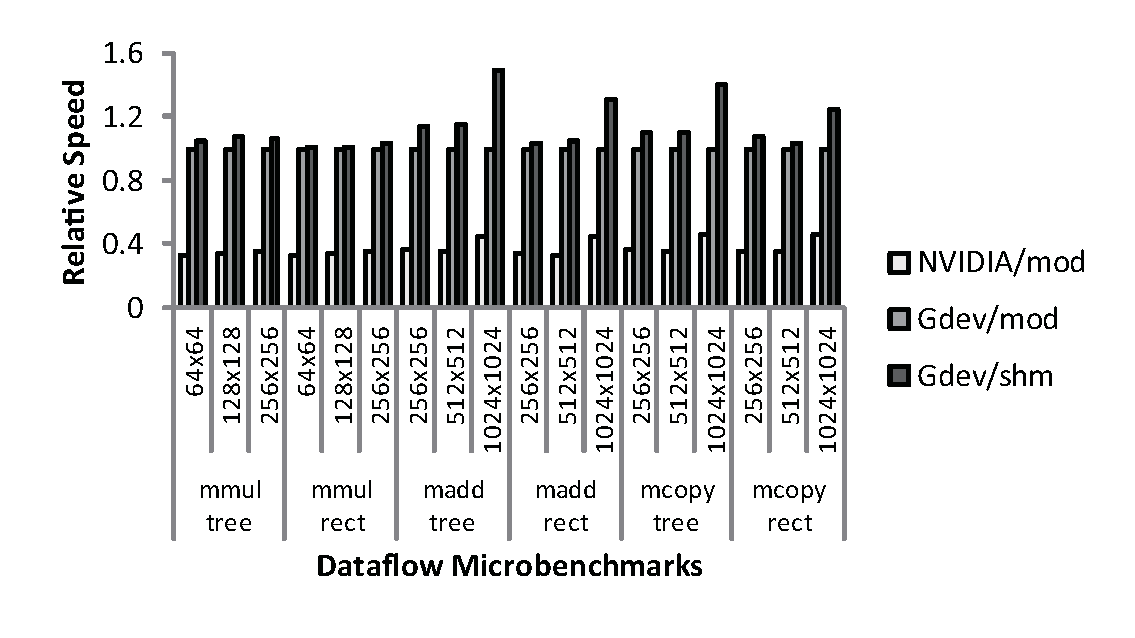
\includegraphics[width=\hsize]{eps/dataflow.eps}\\
  \vspace{-1.5em}
  \caption{Impact of shared memory on dataflow tasks.}
  \label{fig:dataflow}
 \end{center}
 \vspace{-1.5em}
 \begin{center}
  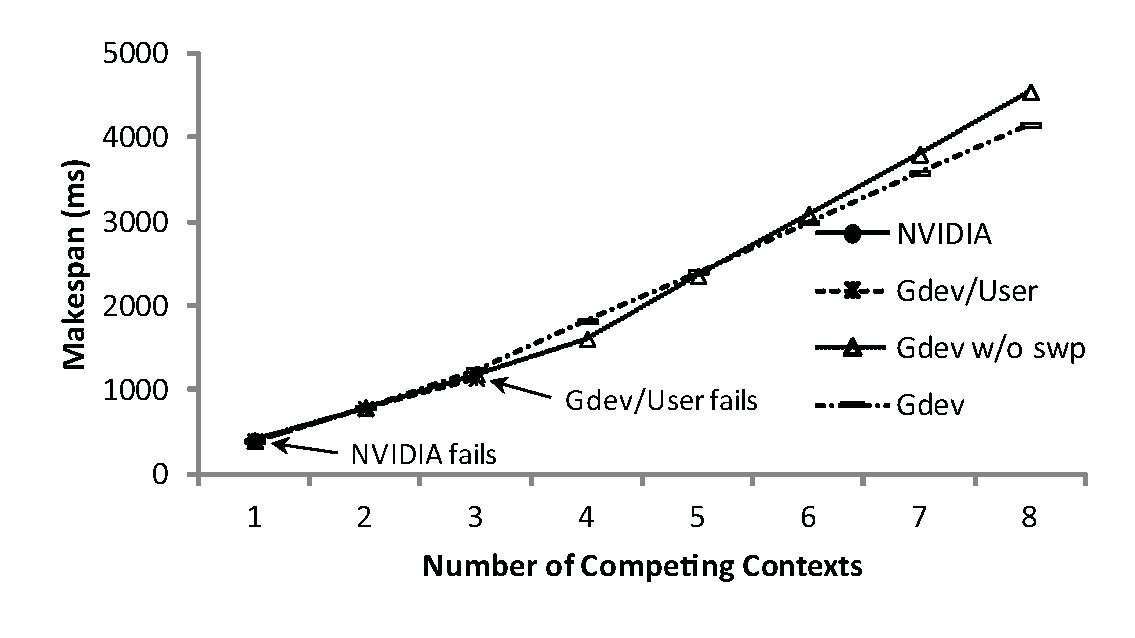
\includegraphics[width=0.75\hsize]{eps/swapping.eps}\\
  \vspace{-1.5em}
  \caption{Impact of swapping latency.}
  \label{fig:swapping}
 \end{center}
 \vspace{-1.5em}
 \begin{center}
  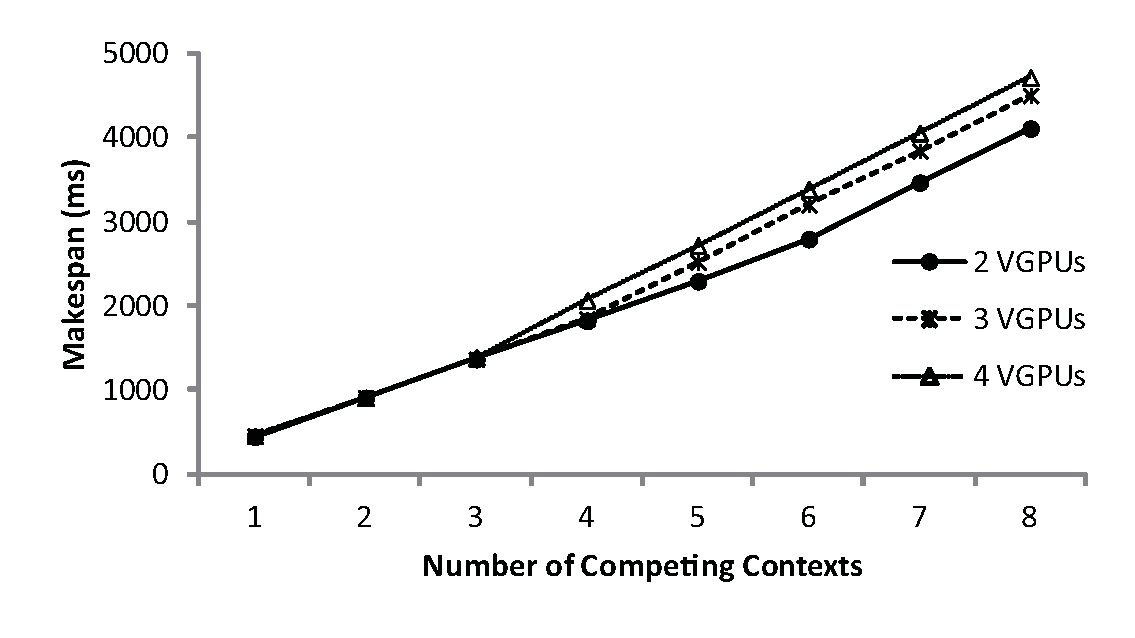
\includegraphics[width=0.75\hsize]{eps/swapping_vgpu.eps}\\
  \vspace{-1.5em}
  \caption{Impact of swapping latency on virtual GPUs.}
  \label{fig:swapping_vgpu}
 \end{center}
 \vspace{-1.5em}
\end{figure}

\begin{figure*}[t]
 \begin{center}
  \subfigure[FIFO scheduler] {
  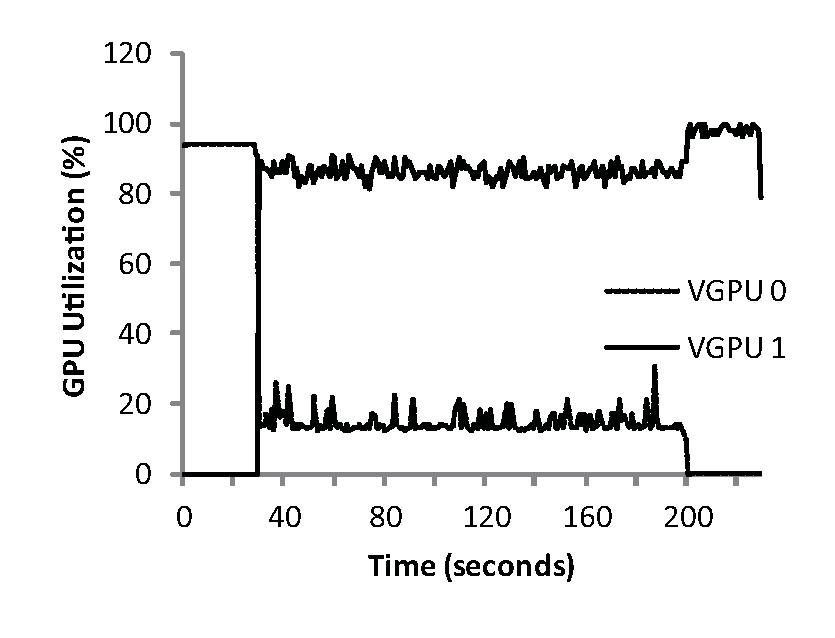
\includegraphics[width=0.318\hsize]{eps/vgpu_2_fifo.eps}
  }
  \subfigure[Credit scheduler] {
  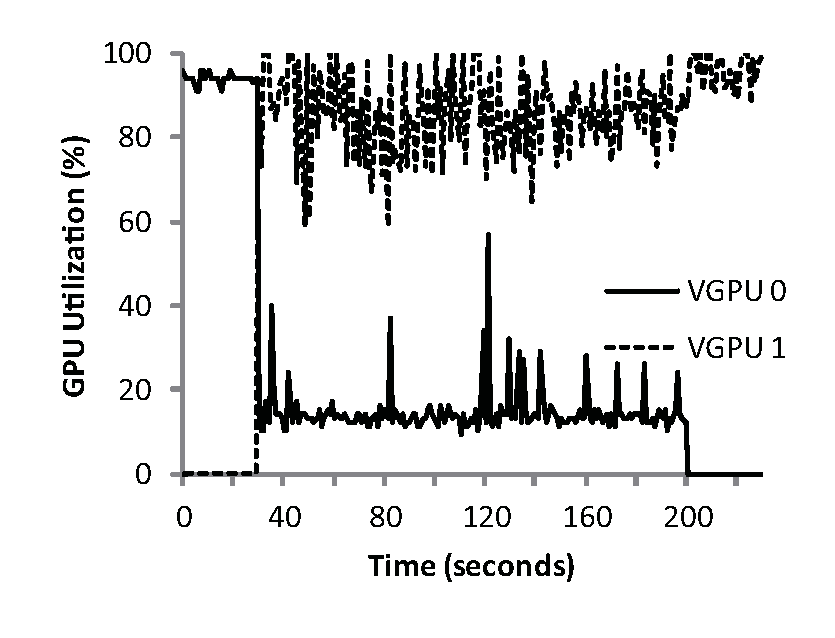
\includegraphics[width=0.318\hsize]{eps/vgpu_2_credit.eps}
  }
  \subfigure[BAND scheduler] {
  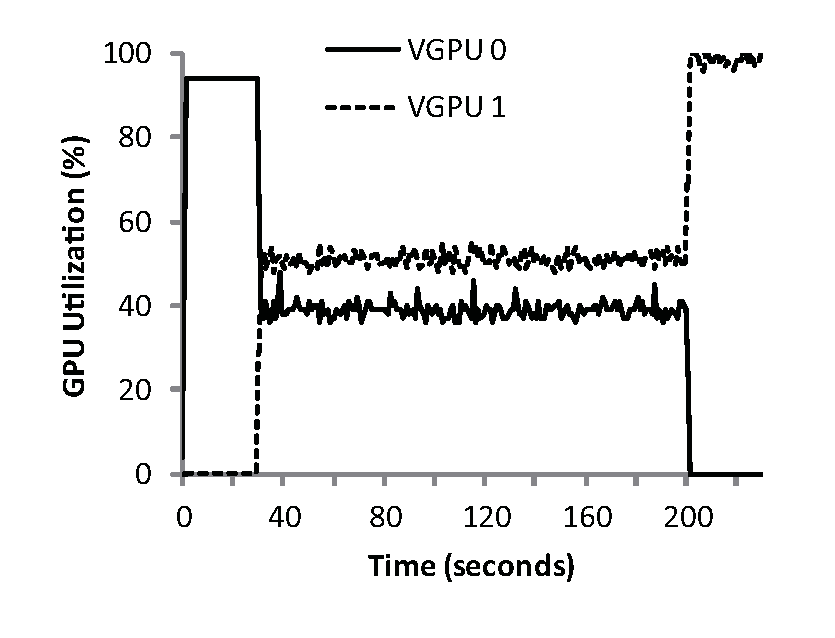
\includegraphics[width=0.318\hsize]{eps/vgpu_2_band.eps}
  }
  \vspace{-1.4em}
  \caption{Util. of virtual GPUs under unfair workloads.}
  \label{fig:vgpu_2}
  \end{center}
  \vspace{-1.5em}
\end{figure*}

Figure~\ref{fig:dataflow} shows the speedups of dataflow benchmarks
brought by Gdev's shared device memory functionality.
Respecting PTask's setup~\cite{Rossbach_SOSP11} for a similar
evaluation, we make a dataflow by a 6x32 tree or a 6x10 rectangle.
``NVIDIA/modular'' and ``Gdev/modular'' use NVIDIA's and Gdev's CUDA
implementations respectively, where a dataflow program is implemented
in such a way that allocates a self-contained context to each graph node
as a module, and connects its output and input by copying data between
host and device memory back and forth.
``Gdev/shm'' uses shared device memory,
\textit{i.e.}, it connects output and input by sharing the same ``key''
associated with the same memory space.
According to the results, shared device memory is fairly effective for
dataflows with large data.
For example, it gains a 49\% speedup for the 1024x1024 madd tree.
Specifically, ``Gdev/modular'' took 1424ms while ``Gdev/shm'' took 953ms
to complete this dataflow. 
This indeed makes sense.
The average data transfer time for a 1024x1024 integer value was about
8ms, and we can reduce data communications by a total of
32+16+8+4+2=62 intermediate nodes for a 6x32 tree, which results in a
total reduced time of 8x62=496ms.
It should be noted that PTask achieves more speedups due to advanced
dataflow scheduling~\cite{Rossbach_SOSP11}.
However, we provide users with a first-class API primitive to manage
shared device memory, which could be used as a generic IPC method to
address different problems.
Therefore, we distinguish our contribution from PTask.
In addition, it is surprising that our prototype system outperforms the
proprietary software significantly.
We suspect that the proprietary one takes a long time to initialize
contexts when there are many active contexts, though an in-depth
investigation is required.

Figure~\ref{fig:swapping} depicts the impact of memory swapping on the
makespan of multiple 128MB-data FAST search tasks, when another 1GB-data
FAST search task runs at the highest priority level. 
Given that the GPU used in this evaluation supports 1.6GB of device
memory, we cannot create more than three 128MB-data search tasks at once
if memory swapping is not provided.
Memory swapping uses shared device memory, which needs access to the
page table.
Hence, our prototype implementation does not support memory swapping as
well as shared device memory for ``Gdev/User'', and it fails when
the number of the small search tasks exceeds three.
It is interesting to observe that NVIDIA' proprietary software fails
when the number of the small search tasks exceeds one.
This is because NVIDIA's proprietary software reserves some
amount of device memory for other purposes.
Unlike the user-space runtime approaches, Gdev's runtime-unified OS
approach can support memory swapping, and all the 128MB-data search
tasks can survive under this memory pressure.
However, a reflection point where the slope of increase in the makespan
changes is different, depending on whether the temporal swap
space allocated on device memory is used or not.
When the temporal swap space is not used, the reflection point is
clearer as observed in ``Gdev w/o swp'', because the swapping latency is
not trivial due to data movement between host and device memory.
Using the temporal swap space, on the other hand, we can reduce the impact
of memory swapping on the makespan of the search tasks, but the
reflection point appears slightly earlier, since the temporal swap space
itself occupies certain space on device memory.

Figure~\ref{fig:swapping_vgpu} shows the impact of memory swapping on
virtual GPUs.
In this experiment, we introduce virtual GPUs, and execute 128MB-data
search tasks on the first virtual GPU.
The memory size available for the virtual GPU is more restricted in
the presence of more virtual GPUs.
We confirm that the makespans become longer and their reflection points
appear earlier for a greater number of virtual GPUs, but all the search
tasks can still complete.
This explains that memory swapping is also useful on virtual GPUs.

\vspace{-0.25em}
\subsection{Isolation among Virtual GPUs}
\vspace{-0.25em}

We now evaluate Gdev in terms of the isolation among virtual GPUs.
Figure~\ref{fig:vgpu_2} demonstrates the actual GPU utilization of two
virtual GPUs, achieved by the FIFO, Credit, and BAND schedulers under
the SDQ scheme.
VGPU~0 executes the LUD benchmark to produce short-length tasks, while
VGPU 1 executes the HW benchmark to produce long-length tasks.
These tasks run repeatedly for 200 seconds to impose high workloads on
the entire system.
To see a workload change clearly, VGPU~1 is started 30 seconds after
VGPU~0.
Our observation is that the FIFO scheduler is not capable of enforcing
isolation at all.
The Credit scheduler also fails to provide isolation, since it is not
designed to handle non-preemptive burst workload.
The BAND scheduler, however, can almost provide the desired GPU
utilization, thanks to the time-buffering policy that allows
short-length tasks to meet the assigned bandwidth.
An error in the utilization of two virtual GPUs is retained
within 7\% on average.

We next study the effectiveness of the MRQ scheme that separates the
queues for compute and memory-copy operations.
Figure~\ref{fig:vgpu_2_band_mrq} illustrates the utilization of two
virtual GPUs under the BAND scheduler, executing the SRAD benchmark
tasks with different sizes of image.
We noticed that the compute and memory-copy operations can be
overlapped, but they affect the run-to-completion time with each other.
When VGPU 1 uses more compute resources due to a large size of
computation, the length of memory-copy operations requested by VGPU 0 is
prolonged due to overlapping.
As a result, it requires more memory-copy bandwidth.
However, the available bandwidth is capped by the BAND scheduler,
\textit{i.e.}, both the compute and memory-copy operations are limited 
to about 50\% of bandwidth at most.
One can also observe that the MRQ scheme allowed the sum of compute and
memory-copy bandwidth to exceed 100\%.

We finally demonstrate the scalability of our virtual GPU support.
Figure~\ref{fig:vgpu_fair_4_band} shows the utilization of four virtual
GPUs under the BAND scheduler, where all virtual GPUs execute four
instances of the LUD benchmark task exhaustively to produce fair
workloads.
The workloads of each virtual GPU begin in turn at an interval of 30
seconds.
Under such sane workloads, our virtual GPU support can provide fair
bandwidth allocations, even if the system exhibits non-preemptive burst
workloads.

\begin{figure}[t]
 \begin{center}
  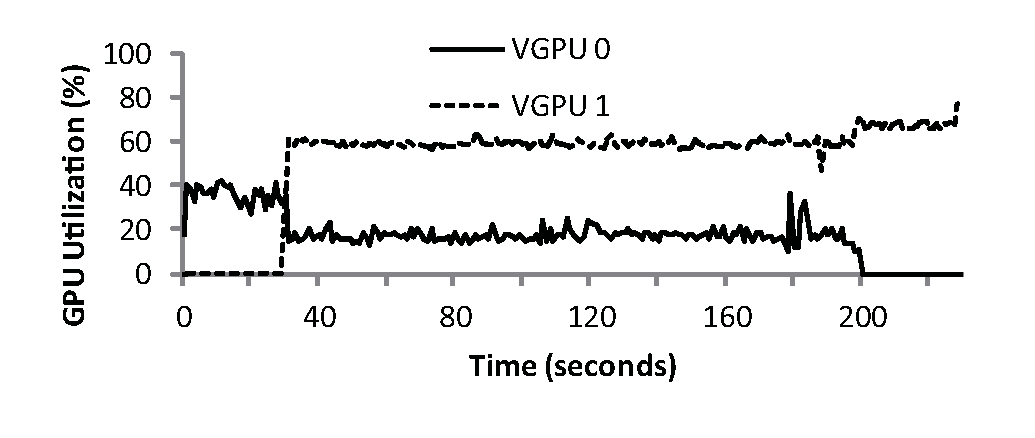
\includegraphics[width=0.93\hsize]{eps/vgpu_2_band_compute.eps}\\
  \vspace{-0.5em}
  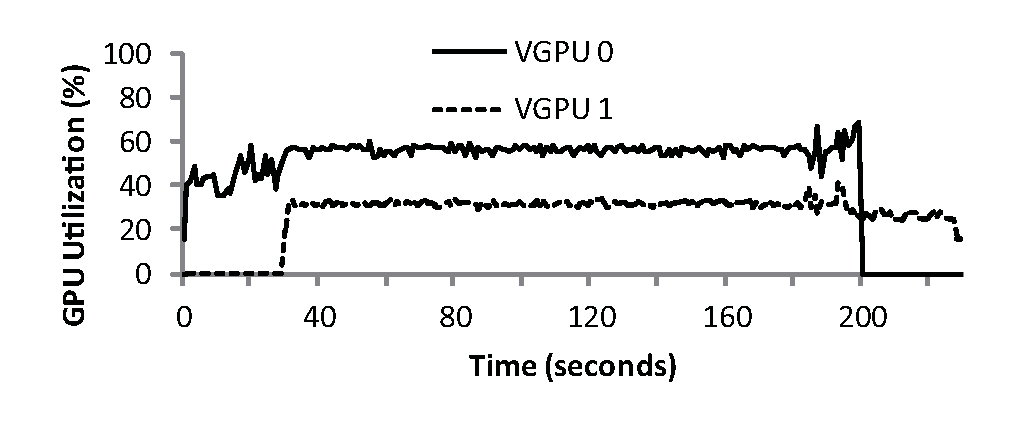
\includegraphics[width=0.93\hsize]{eps/vgpu_2_band_memory.eps}\\
  \vspace{-1.5em}
  \caption{Util. of virtual GPUs with the MRQ scheme (upper for compute
  and lower for memory-copy).}
  \label{fig:vgpu_2_band_mrq}
 \end{center}
 \begin{center}
  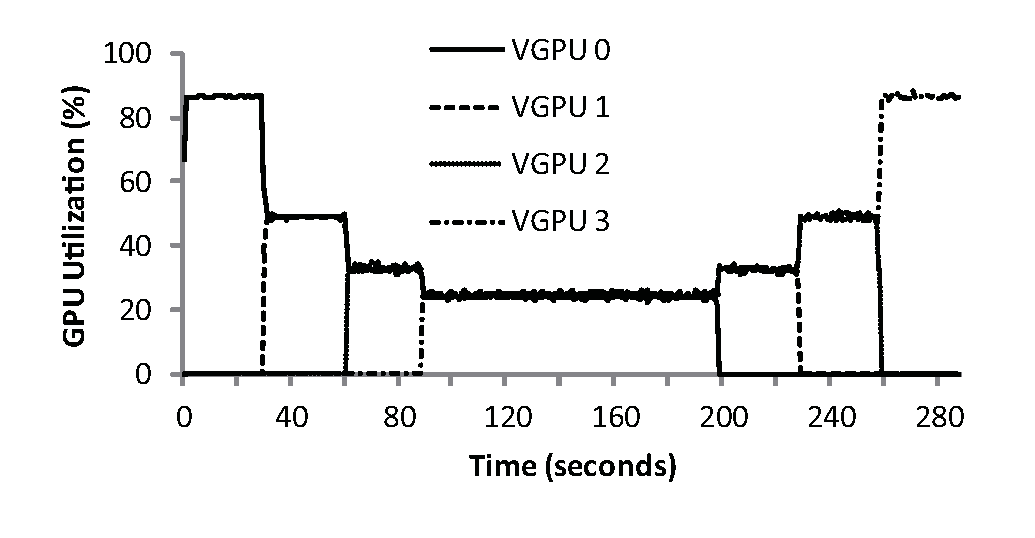
\includegraphics[width=0.93\hsize]{eps/vgpu_fair_4_band.eps}\\
  \vspace{-1.5em}
  \caption{Util. of virtual GPUs under fair workloads.}
  \label{fig:vgpu_fair_4_band}
 \end{center}
  \vspace{-1.5em}
\end{figure}

\section{Related Work}
\label{related_work}

\textbf{GPU Resource Management:}
The GPU is a compute device that essentially requires resource management
to operate.
Recently the research community has developed novel approaches GPU
resource management using OS, runtime library, compiler, and/or
application solutions.

TimeGraph~\cite{Kato_ATC11} and GERM~\cite{Bautin_MCNC08} are GPU
command-driven schedulers integrated in the device driver.
Specifically, TimeGraph provides priority and resource reservation
support for GPU applications, extended with resource sharing
protocols~\cite{Kato_RTAS11}, while GERM addresses fair-share
resource allocation. 
Gdev supports similar scheduling capabilities, but is based on an
API-driven model, where a scheduler is invoked only when tasks use
computing resources on the GPU, eliminating runtime overhead.
A command-driven scheduler also fails to control GPU resource usage
precisely, since it cannot recognize what command sequences would launch
computations on the GPU, and hence it accounts for all commands even
though not using GPU computing resources.

PTask~\cite{Rossbach_SOSP11} is an OS abstraction for GPU applications
to minimize data movement between the host and device memory through
a data-flow programming model.
It also addresses scheduling problems.
CGCM~\cite{Jablin_PLDI11} is a compiler and runtime library solution to
dynamically and automatically optimize host-device data communication,
simiar to PTask.
Gdev does not support such data-flow programming or automatic code
generation; however, it provides programmers with a first-class IPC
primitive for shared memory that can reduce data movement overhead in
communicating with different contexts.

RGEM~\cite{Kato_RTSS11} is a user-space runtime model for real-time
GPGPU applications.
It adovocates split transactions for host-device data transmissions
to bound blocking times, and provides separate queues to demultiplex
schedulers for data transactions and computations.
Although Gdev equips a similar design of separate queues, it
addresses a core challenge of unifying resource management
and runtime support into the OS in order to overcome fundamental
user-space limitations.

In addition to the above differences, Gdev provides virtual GPUs that
enable users to view a physical GPU as multiple logical GPUs for
resource usage isolation.
Furthermore, our design and implementation of Gdev newly developed in
this paper are self-contained, allowing the OS to fully control and even
use GPUs as first-class computing resources, whereas the previous work
more or less depend on the proprietary software or existing graphics
drivers, which forces their solutions, if not concepts, to partly adhere
to user-space runtimes.

\begin{comment}
Comparisons of Gdev and representatives of the above GPU resource
management approaches are summarized in Table~\ref{tab:related_work}.
\begin{table*}[t]
 \caption{Comparisons of Gdev and prior GPU resource management
 approaches.}
 \label{tab:related_work}
 \begin{center}
  {\sf
  \begin{tabular}{|l|p{12.8cm}|}
   \hline
   \hline
  \end{tabular}
  }
 \end{center}
\vspace{-1em}
\end{table*}
\end{comment}


\textbf{GPUs as OS Resources:}
A significant limitation on current GPU programming frameworks is
that GPU applications must reside in the user space.
KGPU~\cite{Sun_SECURITY11_Poster} is a combination of the OS kernel
module and user-space daemon, which allows the OS to use GPUs by
upcalling the user-space daemon from the OS to access the GPU.
On the other hand, Gdev provides OS modules with a set of traditional
API functions for GPU programming, such as CUDA.
Hence, legacy GPU application code can run in the OS without any
modifications and needs not to move back and forth between the user
space and OS.

\textbf{GPU Virtualization:}
VMGL~\cite{Lagar-Cavilla_VEE07} virtualizes GPUs at the OpenGL
API level, and VMware's Virtual GPU~\cite{Dowty_SIGOPS09} exhibits I/O
virtualization through graphics runtimes.
On the other hand, Pegasus~\cite{Gupta_ATC11} uses a hypervisor,
Xen~\cite{Barham_SOSP03} in particular, to co-schedule GPUs and virtual
CPUs in VMs.
Nonetheless, these virtualization systems rely on user-space runtimes
provided by proprietary software, excluding GPU resource management.
In addition, they are mainly designed to make GPUs available in
virtualized environtments, but are not tailored to isolate GPU resources
among users.
Gdev provides virtual GPUs with strong time and space partitioning, and
hence could underlie these GPU virtualization systems.

\textbf{I/O Scheduling:}
GPU scheduling deals with a non-preemptive nature of execution as well
as traditional I/O scheduling.
Several disk bandwidth-aware schedulers~\cite{Gulati_FAST09,
Povzner_EUROSYS08, Wang_FAST07}, for example, contain a similar idea to
the Gdev scheduler.
Unlike typical I/O devices, however, GPUs are coprocessors operating
asynchronously with own sets of execution contexts, registers, and memory.
Therefore, Gdev adopts a scheduling algorithm more appropriate for
compute-intensive workload.

\textbf{Compile-Time and Application Approaches:}
GPU resource usage can be also managed in user application
programs~\cite{Chen_IPDPS10,Guevara09,Saba_RTSS11}, but these approaches
essentially require the programs to be modified or recompiled using
specific compilers and algorithms.
Hence, a generality of programming needs to be compromised.
Under Gdev, on the other hand, applications can use traditional GPU
programming languages.


\vspace{-0.25em}
\section{Conclusion}
\label{sec:conclusion}
\vspace{-0.25em}

This paper has presented Gdev, a new approach to GPU resource management
that integrates runtime support into the OS.
This runtime-unified OS approach realizes new memory management and
scheduling schemes that enable a wide class of applications to GPUs as
first-class computing resources in general-purpose multi-tasking systems.
We implemented a prototype system of Gdev, and conducted thorough
experiments to demonstrate the advantage and disadvantage of using our
Gdev approach. 
Our conclusion is that Gdev needs to compromise some basic performance
due to incorporating runtime support in the OS, but can enhance GPU resource
management for multi-tasking systems and allow the OS itself to use
GPUs for computations.

Our prototype system and application programs used in the performance
evaluation are all open-source, and may be downloaded from our website~\cite{Gdev}.


\renewcommand{\baselinestretch}{0.91}
{\footnotesize \bibliographystyle{acm}
\bibliography{references}}

%\theendnotes

\end{document}
